\documentclass{beamer}

\mode<presentation>
{
  \usetheme{CambridgeUS}      % or try Darmstadt, Madrid, ...
  \usecolortheme{default} % or try albatross, beaver, crane, ...
  \usefonttheme{default}  % or try serif, structurebold, ...
  \setbeamertemplate{navigation symbols}{}
  \setbeamertemplate{caption}[numbered]
} 

\usepackage[english]{babel}
\usepackage[utf8x]{inputenc}

\title[BSP03 - Sortierung ZZ]{Sortierung von Zufallszahlen}
\author{Dickbauer Y., Moser P., Perner M.}
\institute{PS Computergestützte Modellierung, WS 2016/17}
\date{Date of Presentation}

\begin{document}

\begin{frame}
  \titlepage
\end{frame}

% Uncomment these lines for an automatically generated outline.
\begin{frame}{Outline}
  \tableofcontents
\end{frame}

\section{Aufgabenstellung}
\begin{frame}{Aufgabenstellung}

\begin{itemize}
  \item Eingabe: Anzahl an n Zufallszahlen
  \item Erstellung von n Zufallszahlen
  \item Erstellung einer Liste dieser generierten Zufallszahlen
  \item Sortierung dieser Liste Aufsteigend. 1. Priorität nach X, \\2. Priorität: Y
  \item Ausgabe der Liste
\end{itemize}

\end{frame}

\section{Flow Chart}
\begin{frame}{Flow Chart}
	\centering
  	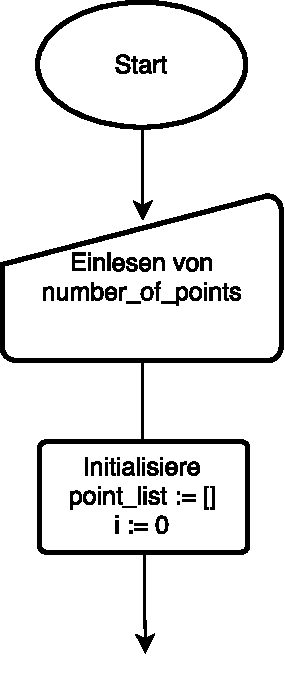
\includegraphics[scale=0.4]{BSP03_Flow_Chart_1.pdf}
\end{frame}
\begin{frame}{Flow Chart}
	\centering
  	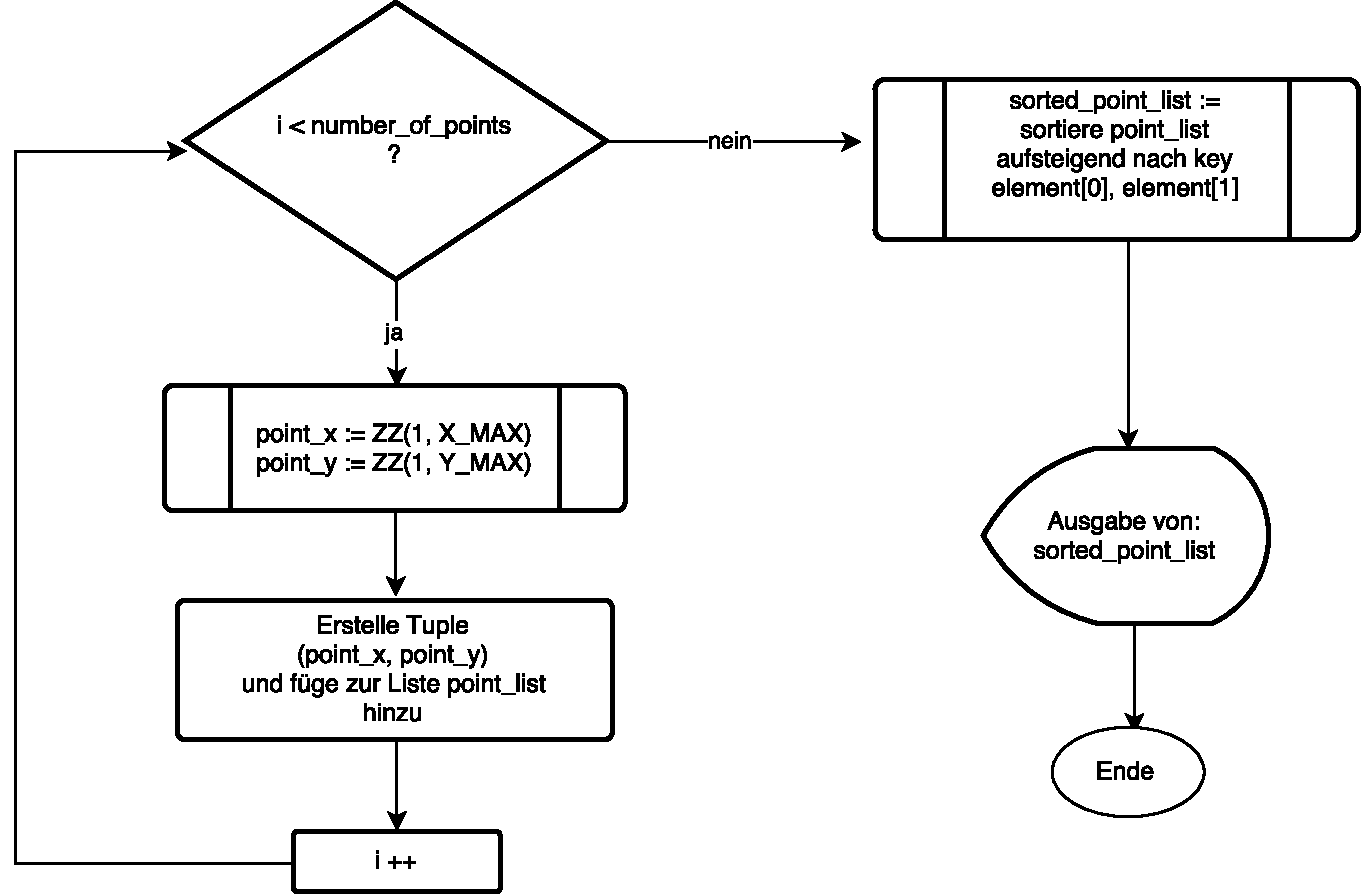
\includegraphics[scale=0.4]{BSP03_Flow_Chart_2.pdf}
\end{frame}

\end{document}
